% !TEX encoding = UTF-8 Unicode
% !TEX spellcheck = de_DE
\documentclass[preprint]{vgtc}               % preprint

\ifpdf%                                % if we use pdflatex
  \pdfoutput=1\relax                   % create PDFs from pdfLaTeX
  \pdfcompresslevel=9                  % PDF Compression
  \pdfoptionpdfminorversion=7          % create PDF 1.7
  \ExecuteOptions{pdftex}
  \usepackage{graphicx}                % allow us to embed graphics files
  \DeclareGraphicsExtensions{.pdf,.png,.jpg,.jpeg} % for pdflatex we expect .pdf, .png, or .jpg files
\else%                                 % else we use pure latex
  \ExecuteOptions{dvips}
  \usepackage{graphicx}                % allow us to embed graphics files
  \DeclareGraphicsExtensions{.eps}     % for pure latex we expect eps files
\fi%

\graphicspath{{figures/}{pictures/}{images/}{./}} % where to search for the images
\usepackage{hyperref} 
\usepackage{microtype}                 % use micro-typography (slightly more compact, better to read)
\usepackage[OT1]{fontenc}
\usepackage[utf8]{inputenc}
\PassOptionsToPackage{warn}{textcomp}  % to address font issues with \textrightarrow
\usepackage{textcomp}                  % use better special symbols
\usepackage{mathptmx}                  % use matching math font
\usepackage{times}
\usepackage[english,ngerman]{babel}                     
\renewcommand*\ttdefault{txtt}         % a nicer typewriter font
\usepackage{cite}                      % needed to automatically sort the references
\usepackage{tabu}                      % only used for the table example
\usepackage{booktabs}                  % only used for the table example

%%%%%%%%%%%%%%%%%%%%%%%%%%%%%%%%%%%%%%%%%%%%%%%%%%%%%%%%%%%%%%%%%%%%%%%%%%%%%%%%%%%%%%%%%%%%%%%%%%%%%%%%%%%%%%%%%%%%%

\onlineid{0}

\vgtccategory{Research}

\vgtcinsertpkg

\preprinttext{Seminar Virtual und Augmented Reality -- WS 2019/20}

\title{Sensorisches Zusammenspiel des visuellen und vestibul\"aren Systems in Virtual Reality}

\author{Nils Henrik Seitz\thanks{e-mail: nils.seitz@uni-rostock.de}\\ \scriptsize Universit\"at Rostock}

\abstract{ Durch die zunehmende Digitalisierung der Gesellschaft, sinkende Kosten und gleichzeitig steigende Leistungsf\"ahigkeit der erfordlichen Hardware erfreut sich Virtual Reality immer gr\"oßerer Beliebtheit.
} 


\CCScatlist{ 
	\CCScat{H.1.2}{Models and Principles}{User/Machine Systems}{Human factors, Human information processing};
	\CCScat{H.5.1}{Information Interfaces and Presentation (e.g., HCI)}{Multimedia Information Systems}{Artificial, augmented, and virtual realities}}

\keywords{Visual-vestibular conflict, motion sickness, cyber sickness, multisensory integration}

% Make Structure(section, sub(sub)sections, enumerate/itemize, figures and tables (see original for formatting (LABEL THEM, do captions, width and centering)), <- AUTOREF, make cites (FROM BIBDESK!!) and footnotes, sparsely use texttt / -it / -bf, use good latex style (symbols, equtions, etc.) and good indentation!)

%% FIGURES
%\begin{figure}[tb]
%	\centering % avoid the use of \begin{center}...\end{center} and use \centering instead (more compact)
%	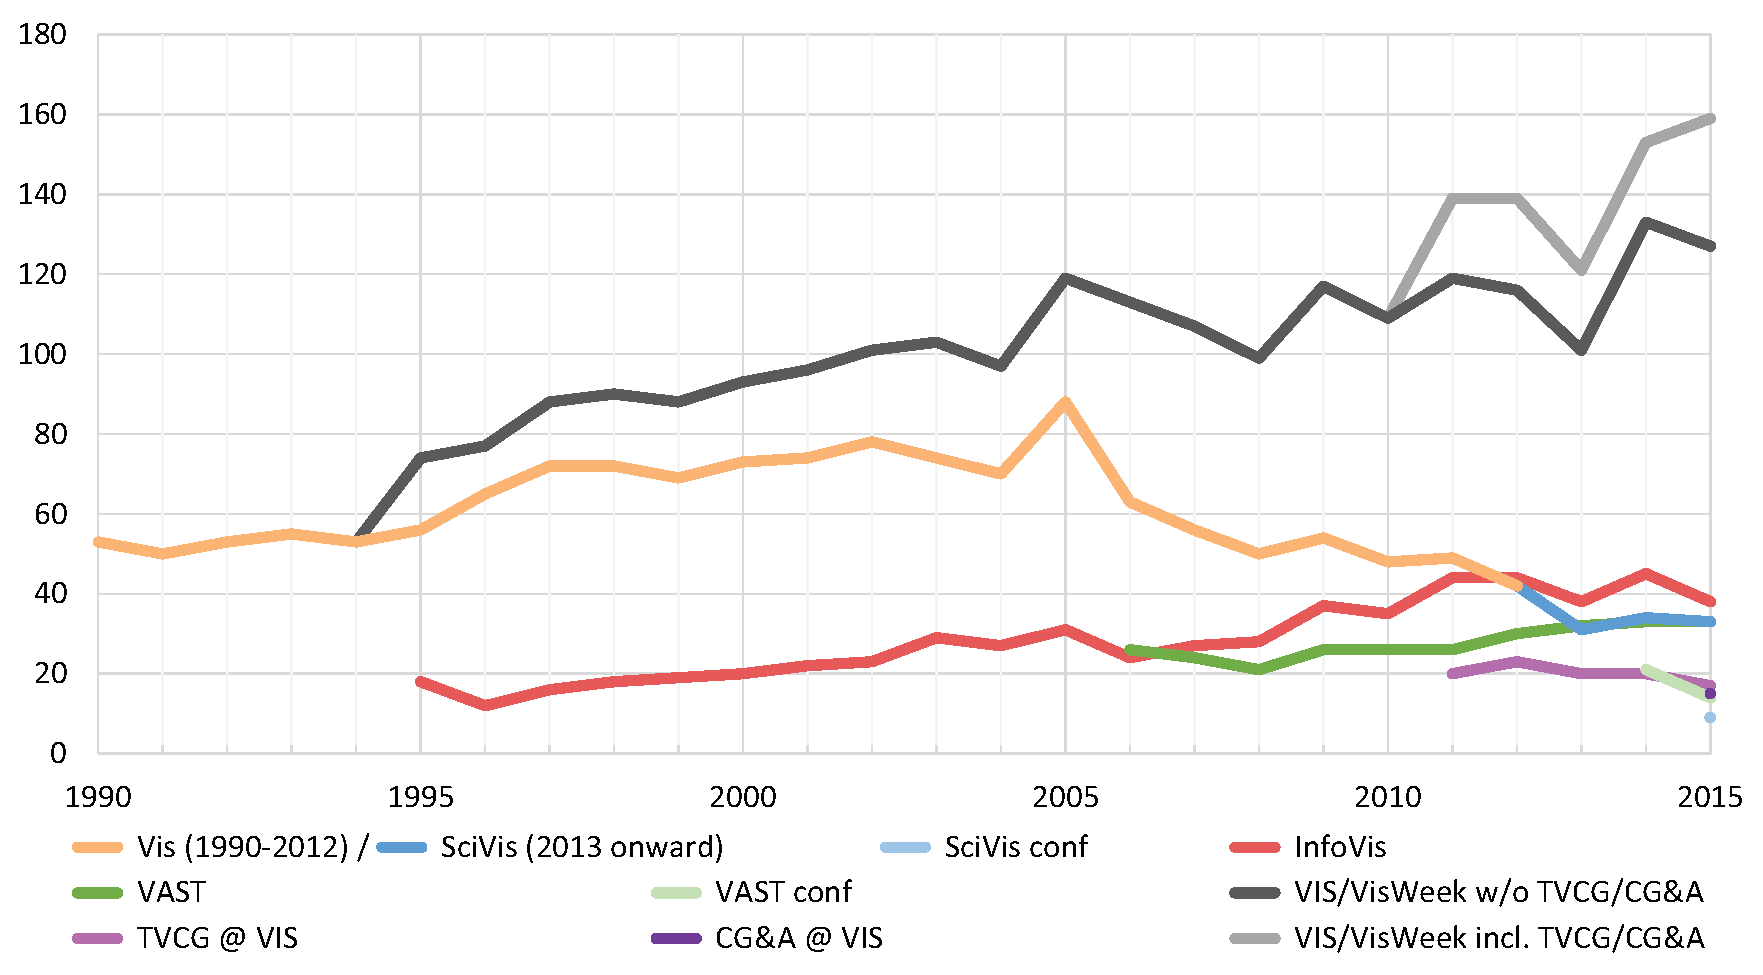
\includegraphics[width=\columnwidth]{paper-count-w-2015-new}
%	\caption{A visualization of the data from \autoref{tab:vis_papers}. The image is from \cite{Isenberg:2017:VMC} and is in the public domain.}
%	\label{fig:sample}
%\end{figure}

\begin{document}

\maketitle

\section{Einleitung} 
	Evolution\"ar gesehen, ist es die gr\"o{\ss}te St\"arke des Menschen, sich seiner Umgebung oder auch seine Umgebung an sich anzupassen. Daher liegt es in der Natur des Menschen, sich Werkzeuge herzustellen und Erfindungen zu machen, die im Alltag hilfreich sind.

Eine der wichtigsten Grundlagen daf\"ur ist die multisensorische Integration, ein evolution\"ares Wunder f\"ur sich, denn sie erm\"oglicht ein hohes, abstraktes Verst\"andnis und die F\"ahigkeit zu lernen. Unser Gehirn f\"uhrt unbemerkt und scheinbar m\"uhelos mehrmals innerhalb einer Sekunde die Informationen verschiedener Sinne zu einem f\"ur uns konsistenten Gesamtbild zusammen.
Dass diese Verarbeitung \"uberhaupt stattfindet, ist uns selten bewusst\cite{Deroy:2016:SensInte}. Sobald es dabei aber zu Komplikationen, das hei{\ss}t, Abweichungen der bisherigen Erfahrung, kommt, bemerken wir dies sofort. 

Eine relativ neue Erfindung ist Virtual Reality, mit der wir erstmalig die Chance haben, unsere Umgebung vollst\"andig nach unseren Vorstellung zu formen, beispielsweise auch mit ver\"anderten physikalischen Gesetzen.
Virtual Reality hat das enorme Potential, viele Bereiche der Gesellschaft nachhaltig zu ver\"andern, nur trifft es sich leider, dass genau bei der Integration der Sensorik Schwierigkeiten auftreten, die als Cyber Sickness bekannt sind.

\section{Cybersickness}
	Das gravierendste Problem, welches bei der Nutzung von Virtual Reality auftreten kann, sind die Symptome der Cyber Sickness. Diese ähneln denen der klassischen Motion Sickness und umfassen eine Vielzahl unangenehmer Empfindungen und Reaktionen durch den betroffenen Organismus: Kopfschmerzen, Schweißausbrüche, Orientierungslosigkeit, Schwindelanfälle, Ataxia und Übelkeit bis hin zum Erbrechen\cite{LaViola:2000:CSinVR, Kolasinski:1998:SympCS}.\\
Durch die Ähnlichkeit in den körperlichen Reaktionen zur klassischen Motion Sickness, die beispielsweise von Auto- oder Schifffahrten bekannt ist, versucht man auch, denselben Erklärungsansatz zu verwenden: die \textit{Sensory Conflict Theory}\cite{Kolasinski:1998:SympCS,Johnson:2005:SCT_Expl}.
Diese postuliert, dass die Symptome auftreten, wenn bei der multimodalen, sensorischen Integration bezüglich der Selbstbewegung inkongruente Reize wahrgenommen wurden und vor allem dann, wenn das aktuelle Empfinden im Widerspruch mit vorherigen Lernerfahrung in ähnlichen Situationen steht\cite{Reason:1975:MSexp}.\\
Für die Wahrnehmung von Bewegung ist die Propriozeption, vor allem aber der Gleichgewichtssinn und Sehsinn zuständig.
Bei Motion Sickness besteht das Problem darin, dass keine passenden visuellen Reize vorhanden sind, wie auf der Innenkabine eines Schiffes bei starkem Wellengang, was bekanntermaßen zu Seekrankheit, eine Form der Motion Sickness, führt.
Im Gegensatz dazu entsteht bei Virtual Reality \textit{Vection}, eine Illusion in der Perzeption der Eigenbewegung, die allein durch visuelle Stimuli entsteht, ohne vestibuläre Stimuli.\\
Zwar liegt beiden, Motion und Cyber Sickness, der \textit{visuell-vestibuläre Konflikt} zu Grunde, jedoch ist die Art, wie dieser entsteht, ebenso wie einige Symptome der beiden, unterschiedlich \cite{Stanney:1997:MSCSSS}. Deswegen wird die Sensory Conflict Theory auch durchaus als Erklärung für die Symptome der Cyber Sickness angezweifelt  \cite{Kolasinski:1998:SympCS}.\\
Eine Alternative stellt die \textit{Theory of Postural Instability} dar:

\section{Methoden}
	test

\section{Ergebnisse}
	test

\section{Fazit}
	Cyber Sickness entsteht durch eine Form des visuell-vestibul\"aren Konflikts und ist, auf Grund der entstehenden Symptome, ein zentraler Aspekt der Nutzung von Virtual Reality. Diese k\"onnen das Erlebnis in einer virtuellen Realit\"at unertr\"aglich machen.

Es wurden in \autoref{Maßnahmen gegen CS} eine Reihe verschiedener Methoden vorgestellt, mit deren Hilfe man, vor allem durch Kombination der Methoden und unter Beachtung bestimmter Faktoren, Cyber Sickness reduzieren kann. Das generelle Prinzip der Nat\"urlichkeit oder Vertrautheit, das es einzuhalten gilt, zieht sich durch die Ma{\ss}nahmen.
Dieses Wissen kann helfen, in Zukunft einen besseren, f\"ur den Anwender angenehmeren Umgang mit weniger Cyber Sickness-Symptomen in Virtual Reality zu erm\"oglichen. Dennoch haben diese Methoden nur bedingte G\"ultigkeit und \"Ubertragbarkeit, da es sich hierbei noch um Grundlagenforschung handelt.

Es ist wichtig zu verstehen, dass momentan keine Theorie existiert, die die Ph\"anomene von Cyber Sickness vollst\"andig erkl\"aren kann. Daher ist es auch nicht m\"oglich zu sagen, ob Cyber Sickness und klassische Motion Sickness denselben Ursprung haben. Dennoch beziehen sich viele Studien \"uber Cyber Sickness in Virtual Reality auf \"altere Studien, in denen es eigentlich um klassische Motion Sickness oder Simulator Sickness geht und versuchen, \"ahnliche Ergebnisse im Sinne der Sensory Conflict Theory zu finden. Dies hat oft widerspr\"uchliche Ergebnisse zur Folge.

Weiterhin folgt aus dieser "`Vererbung"' von der klassischen Motion Sickness an die Cyber Sickness, dass in der Literatur keine eindeutige Nomenklatur herrscht, in der Begriffe wie Cyber Sickness, Virtual Reality Sickness, Simulator Sickness und Motion Sickness teils synonym verwendet werden, ohne dass dies gerechtfertig ist, da es keine genauen Definitionen f\"ur die jeweiligen Begriffe gibt.

Ausgehend von einer exakteren Benennung wird dann zus\"atzliche Forschung ben\"otigt, um eine bessere Theorie zur Erkl\"arung von Cyber Sickness zu finden. Auch m\"ussen neue Messverfahren erschlossen werden, da viele der Messung aktuell auf Selbstausk\"unften beruhen, welche subjektiv verf\"alscht sein k\"onnen. Durch Umsetzen dieser drei Punkte w\"urden danach eindeutigere, weniger widerspr\"uchliche und vor allem besser vergleichbare Ergebnisse entstehen. Es ist wichtig, dies nicht zu vernachl\"assigen, w\"ahrend in der Zwischenzeit mit den aktuellen Gegebenheiten weitergeforscht wird.

Zuletzt sollte bei zuk\"unftiger Forschung und der Umsetzung neuer Methoden an verschiedenste Gruppen gedacht werden, damit keine Ungleichheit zwischen Gruppen herrscht, wie das bei der Passform der Head-Mounted Displays in \autoref{abb:hmdfit} der Fall war. Der Mensch hat sich in seiner Evolution \"uber die Zeit schon an verschiedenste Gegebenheiten angepasst, somit ist anzunehmen, dass selbiges auch f\"ur Virtual Reality gilt. Bis dahin m\"ussen wir uns aber selbst bestm\"oglich unterst\"utzen, durch eben genannte Verbesserung und mit Methoden gegen Cyber Sickness, damit wir das gro{\ss}e Potential, welches Virtual Reality innewohnt, effektiv nutzen k\"onnen.


\section*{Danksagung}{
	Der Autor m\"ochte Amon Ties Uerckwitz f\"ur die Zusammenarbeit im Themengebiet "`Human Factors and Perception"' danken.}

\bibliographystyle{abbrv-doi-hyperref-narrow}
\bibliography{sources}
\end{document}
